\addchap{Anhang}
\label{chap:appendix}

\addsec{Beispiel-Produktanfrage}
\label{appendix:inquiry}

Der folgende Text ist eine Beispiel-Produktanfrage. Er kann automatisch
von \name bei der Erstellung einer Produktanfrage generiert werden.\\
Dabei werden \texttt{<productname>}, \texttt{<gtin>} und \texttt{<name>}
durch die entsprechenden Angaben ersetzt.

Die Hinweise am Ende der E-Mail werden immer angehängt und können
nicht verändert werden.

Der Text wurde mit Hilfe des Baukastensystems der
Tierrechtsorganisation Maqi erstellt \citeweb{maqi:inquiry}.

\begin{verbatim}
Sehr geehrte Damen und Herren,

ich lebe aus ethischen Gründen vegan, vermeide also alle
Tierprodukte.
Da dennoch in einem Produkt neben offensichtlichen Tierprodukten wie
Milch, Rinderfett etc. auch versteckte Tierprodukte oder Zutaten, die
sowohl von Tieren als auch von Pflanzen stammen können (beispielsweise
Mono- und Diglyceride von Speisefettsäuren, Vitamine, Aromastoffe
etc.) enthalten sein können, würde ich gerne wissen ob ihr Produkt
"<productname>" mit der GTIN <gtin> wirklich vegan
ist.

Bitte teilen Sie mir mit:
* Welche Zutaten werden verwendet (auch solche, die laut Gesetz keine
sind bzw. nicht deklariert werden müssen)?
* Woraus sind die zusammengesetzten Zutaten zusammengesetzt (sofern
nicht angegeben)?
* Woraus sind die synthetisierten Zutaten synthetisiert (z.B. kann
Vitamin D aus Lanolin, Wollfett synthetisiert sein, welches nicht
vegan ist)?
* Welche Produktionshilfsstoffe werden verwendet (auch wenn diese im
Endprodukt nicht mehr oder kaum noch vorhanden sind)?
* Welche entsprechenden Aussagen gelten für die Verpackungsmaterialien
(beispielsweise kaseinhaltigen Kleber für die Etikettierung)?

Sollten Sie weitere potentiell vegane Produkte herstellen, würde ich
entsprechende Informationen darüber natürlich ebenfalls begrüßen.

Für Rückfragen stehe ich gern zur Verfügung.
Im Voraus vielen Dank für Ihre Bemühungen.

Mit freundlichen Grüßen,
    <name>

Hinweise
========

Dies ist eine automatisch erstellte Mail von 
http://yava.yhaupenthal.org/.

Es ist wichtig, dass Sie nicht den Betreff ändern, insbesondere
nicht die Zahl, um eine automatische Einsortierung zu ermöglichen.

Bitte achten Sie darauf, dass Ihre Antwort veröffentlicht wird, Sie
geben mit einer Antwort damit also Ihr Einverständnis, wobei Ihre
Daten anonymisiert werden können. Bitte teilen Sie dies mit.
\end{verbatim}

\addsec{Datenbank}
\label{appendix:db}

Das Datenbankmodell, welches in Abbildung~\ref{pdf:erd} zu sehen ist,
zeigt alle Tabellen mit den jeweiligen Spalten von \name in der
Übersicht und wie diese Tabellen miteinander verknüpft sind.

Das Modell wurde mit Hilfe des Ruby-Gems "`railroady"' erstellt.

% railroady -b -l -M > important_models.dot

\begin{sidewaysfigure}
  \centerline{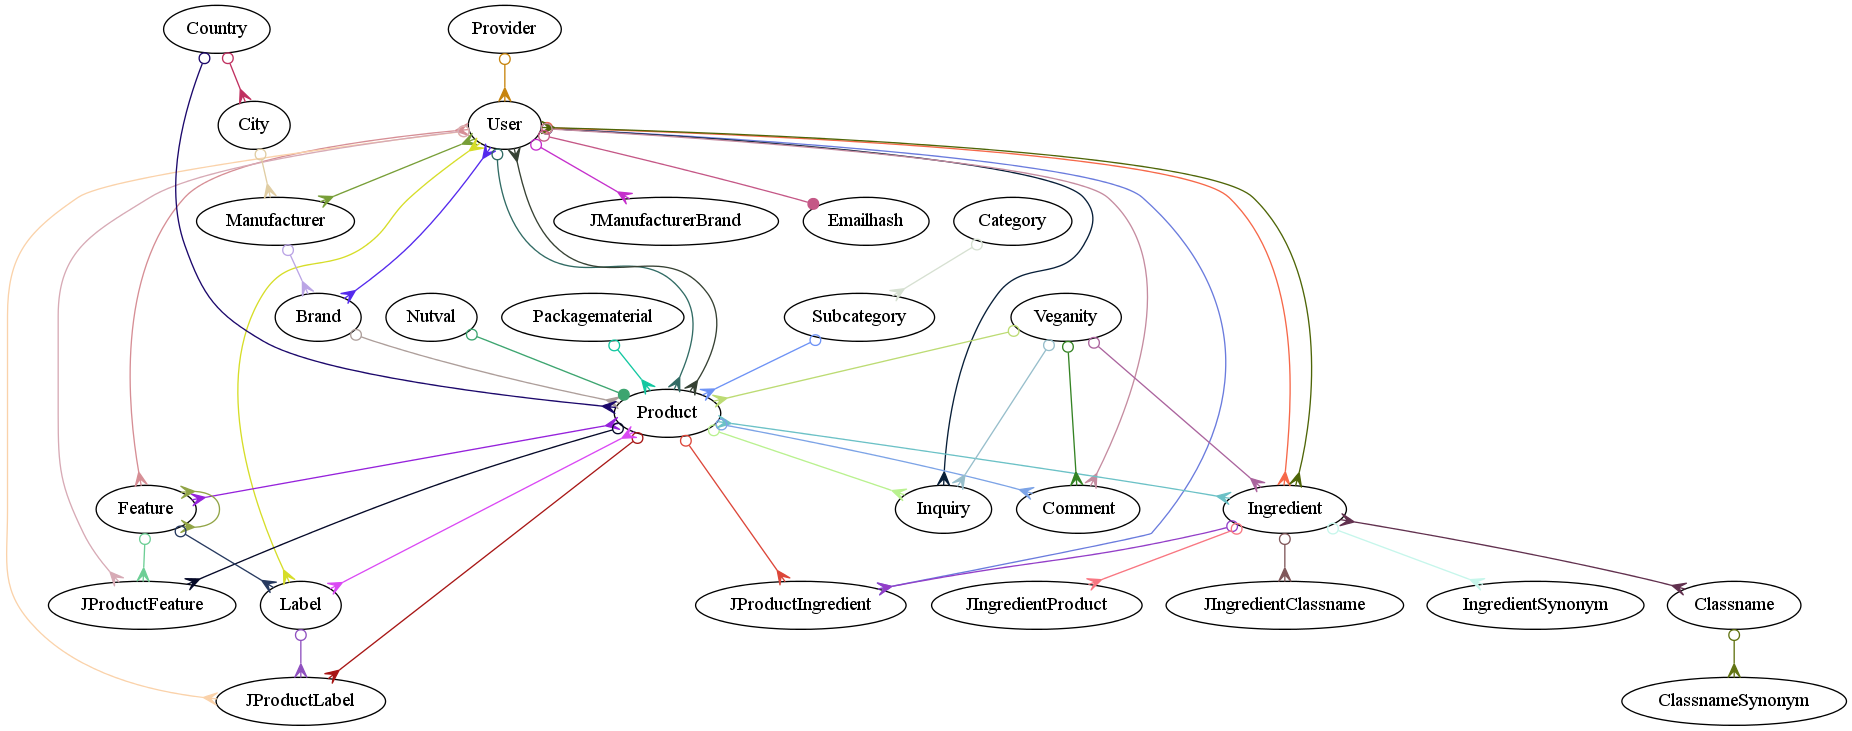
\includegraphics[scale=0.4]{misc/important_models.png}}
  \caption{Entity-Relationship-Modell von \name}
  \label{pdf:erd}
\end{sidewaysfigure}